\documentclass[10pt,english,a4paper]{article} %twosided
\usepackage[utf8]{inputenc}
\usepackage{graphicx}
\usepackage{url} 
\usepackage{hyperref} 
\usepackage{cite}
%\usepackage{times}
\pagestyle{headings}

\title{Improving computer science and software 
engineering education in cyberlearning 
environments through understanding UI and UX design
\thanks{Semestrálny projekt v predmete Metódy inžinierskej práce,
 ak. rok 2020/21, vedenie: Martin Sabo}}

\author{Márk Bartalos \\[2pt]
        \small{Slovak University of Technology in Bratislava}\\
        \small{Faculty of Informatics and Information Technologies}\\
        \small{\texttt{xbartalosm@stuba.sk}}
}

% \date{\small 30. september 2020}


\begin{document}

\maketitle

\begin{abstract}
    In our day and age cyberlearning for computer science and software engineering education has become more popular than ever.
    Thanks to its growing popularity and adoption rate, online cyberlearning environments (CLE) are advancing very quickly.
    In order to make these CLEs as effective and user-friendly as possible we need to understand how their design
    works and what common problems can occur. This article will offer possible testing solutions for analyzing and testing
    the design of complex CLEs and web tools targeted for computer science (CS) and software engineer (SE) students. 
    It will give a better understanding what exactly is meant under the terms ``UI/UX" and will list possible solutions that
    can be implemented to improve current environment designs, leading to improvement in teaching these field.
% The article will be about how understanding UI and UX design principles can serve as a basis for future improvements in teaching
% these fields. My goal is to understand UI/UX design techniques to be able to identify the problems with currently 
% implemented cyberlearning environment designs. The identified problems then could be used to improve already existing environments.
% Knowledge of these problems would be greatly beneficial in the design and development of new, learning focused, student 
% oriented cyberlearning environments for computer science (CS) and software engineering (SE) students.
\end{abstract}



\section{Introduction}
We speak about distance learning from around two centuries ago\cite{moore_2011_elearning}, under which
I am referring to learning through online environments. What distance learning really means is highly debated\cite{moore_2011_elearning},
but I believe it can also refer to learning through online environments, because lot of authors use learning through and online environment and distance learning as
synonyms\cite{distance_definition}\cite{moore_2011_elearning}. 
Now distance learning is becoming a necessity rather than an option. Especially in the middle of a pandemic, use of online 
education environments have become more needed than ever. This article will focus on online cyberlearning environments 
mainly designed for computer science (CS) and software engineer (SE) students.
% Implementing cyberlearning 
% environments for teaching these fields can be the more beneficial than implementing it in teaching for non computer 
% related fields. 


The used terms will be defined in the definitions section \ref{definitions}.
Methods that could be used will be explored more in section ``Methods for analysis" \ref{methods}.
I will talk more about the most common problems with the currently implemented cyberlearning environment (CLE)
designs in the ``Common problems section" \ref{problems}.


\section{Definitions}\label{definitions}

\subsection{Cyberlearning}
For cyberlearning I will use the definition by National Science Foundation: 
``the use of networked computing and communications technologies to support learning” \cite{borgman_2017_fostering} 
Cyberlearning itself can be form of distance learning, but its main focus is building an all 
encompassing online environment which can motivate, inspire and and teach students using 
computer systems and networking technologies as primary tools. \cite{ui/ux}
Primary goal of cyberlearning is to provide learning experiences via a technology-based platform. 
Cyberlearning in some way is an extension of and a twist on e-learning \cite{lynch_2020_cyberlearning}.
While e-learning refers to how the content is delivered, in cyberlearning, technology
is used to carry out learning experiences which would be otherwise impossible without technology \cite{lynch_2020_cyberlearning}.

\subsection{Cyberlearning env. for CS and SE students}
Under the term ``Cyberlearning environments for computer science and software engineer students', I am mainly
referring to an online CLE which enable students to write and compile code online. These are all encompassing
environments, meaning they are equipped with 
online compilers and debugging tools, so students don't require any additional software to be installed on their PC, making
the whole programming experience more accessible for everyone.
With the help of these kind of CLEs students are able to learn the curriculum through lectures and practice
what they have learnt, with only requiring a web browser.

\subsection{User Interface (UI)}
UI and UX are often confused terms. \cite{theymakedesign_2019_what} They have similarities, but in reality
these are completely different things.
UI stands for User Interface. User Interface design defines the graphical layout of the page or application.
User interface designers are responsible for defining the how each element will look, their size and position.
Its their job to make the look and feel of the page or application aesthetically pleasing and 
attractive. Animation, transition design, choosing of the correct fonts and images also part of the UI design, 
these have to be designed such a way that they are in harmony and logically connected to each other.
\cite{theymakedesign_2019_what}

\subsection{User Experience (UX)}
UX stands for ``user experience". UX designers are also concerned with the User interface\cite{theymakedesign_2019_what}. 
The main difference between UI and UX is that while UI focuses on the look of the application,
UX focuses on the functionality and interactions of the application. UX designers are 
responsible form making sure the User Experience is intuitive and can be easily understood by everyone.
They have to make sure that the connection between different parts are organized in a logical way.
UX designers are also have to have and understanding of how users interact with their
device so that the UX can be easy to use and user friendly\cite{theymakedesign_2019_what}. 

\section{Importance of UI/UX design}\label{importance}
Design of the environment has a big role in the effectiveness and in 
its ability to properly convey information \cite{ui/ux}. 
By a study done in 2002 called "Usability evaluation of web-based learning", we know that User interface
has reasonable impact on the student's behavior while using the environment\cite{wesson_2002_usability}.
The study concluded that students preferred the environment which provided a consistent experience and could be navigated more easily
\cite{wesson_2002_usability}. That is why its necessary to create CLEs that can be easily navigated,
where information and tools are arranged into logical groups and have a consistent user-friendly design.


% \begin{figure}
%     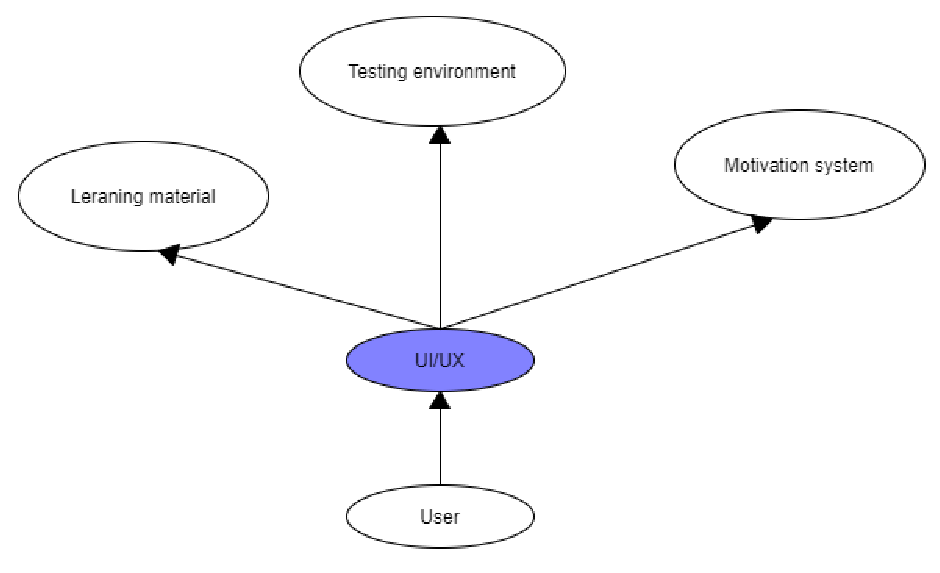
\includegraphics[width=1\textwidth]{images/diagram-crop.pdf}
%     \caption{Diagram illustrating the role of UI/UX in CLE}
% \end{figure}


\section{Methods for analysis}\label{methods}
There are several methods for testing UI/UX design of online environments. The testing 
can be automated or done by a group of people manually.

\subsection{Automated testing}
Automated testing of UI is a relatively new thing.\cite{automated_testing_ifml} There aren't many well known methods
providing fully automatic testing of a web environment, but a recent study shows that
it is possible using Interaction Flow Modeling Language (IFML) Models.\cite{automated_testing_ifml}
IFML is evolved from WebML and its designed to capture the structure, user interaction and control
flow of front-end of web applications.\cite{automated_testing_ifml}.
To automate and validate the UI design the developers have to create an IFML model
of the front-end. In order to design an IFML model, an UML (Universal Modelling Language) model 
containing the domain concepts of the application is required.\cite{automated_testing_ifml}. 
When the IFML and the UML models are completed they have to be processed by an application written 
in Java, which will generate a Test case document (.txt), a Navigation Modell (.xta) and the State Transition 
Matrix (.xls). Then the generated data can be used to analyze and easily spot flaws with the web application, like bad navigation design
\cite{automated_testing_ifml}. 
Thanks to usage of generalized Markup Languages this application can be used for all kind of web environments. 
By using this program we could analyze our web based CLEs for CS and SE students. 
The produced data then could be used to improve their layout, remove confusing elements and improve the usability of the design,
making the learning process more efficient.


\section{Most common problems}\label{problems}

% \section{Possible solutions}

\section{Conclusion}





% Motivujte čitateľa a vysvetlite, o čom píšete. Úvod sa väčšinou nedelí na časti.

% Uveďte explicitne štruktúru článku. Tu je nejaký príklad.
% Základný problém, ktorý bol naznačený v úvode, je podrobnejšie vysvetlený v časti~\ref{nejaka}.
% Dôležité súvislosti sú uvedené v častiach~\ref{dolezita} a~\ref{dolezitejsia}.
% Záverečné poznámky prináša časť~\ref{zaver}.




% \begin{figure}
% 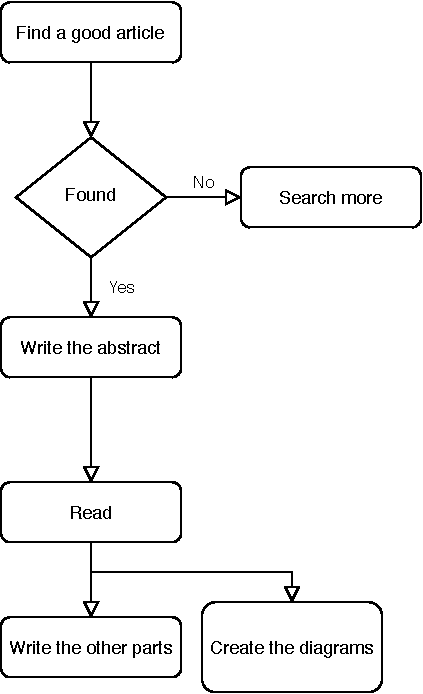
\includegraphics[width=0.75\textwidth]{images/flowchart-crop.pdf}
% \end{figure}
% \section{Nejaká časť} \label{nejaka}

% Z obr.~\ref{f:rozhod} je všetko jasné. 

% \begin{figure*}[tbh]
% \centering
% %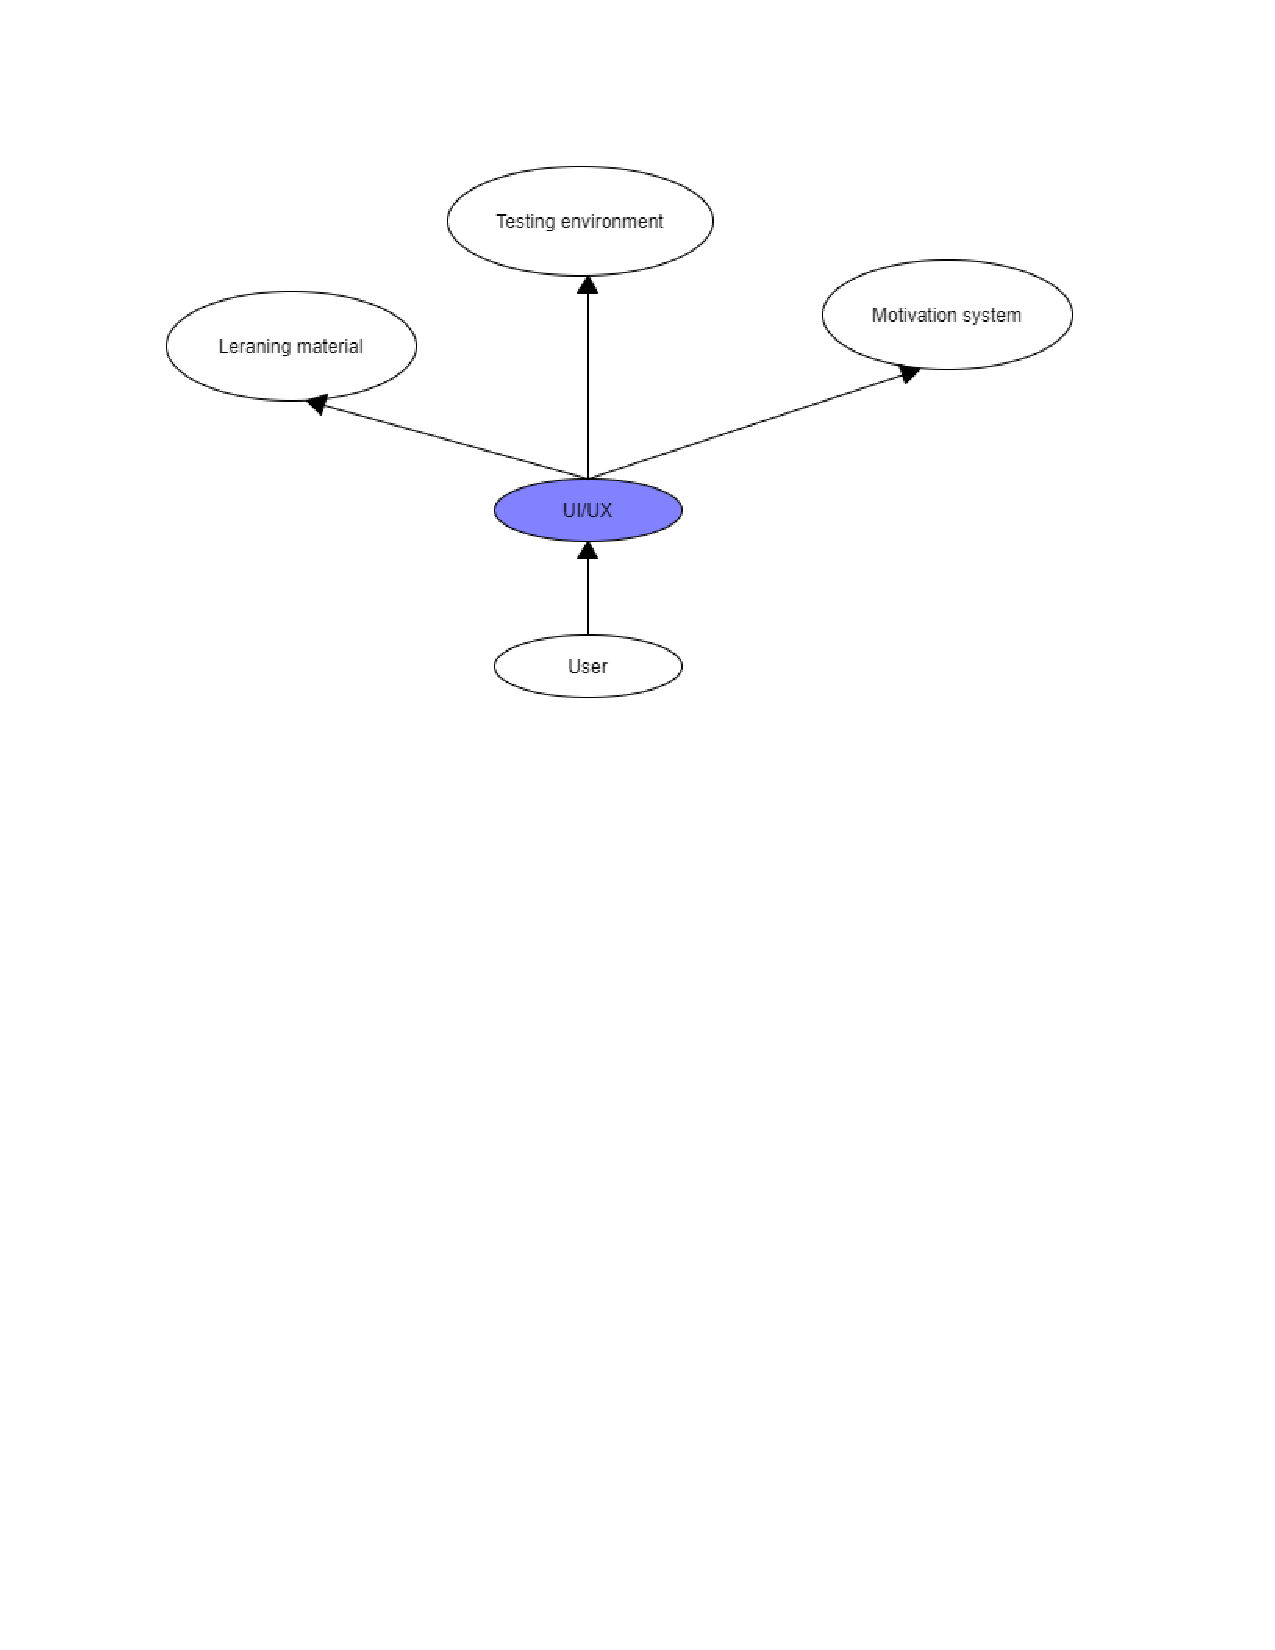
\includegraphics[scale=1.0]{diagram.pdf}
% Aj text môže byť prezentovaný ako obrázok. Stane sa z neho označný plávajúci objekt. Po vytvorení diagramu zrušte znak \texttt{\%} pred príkazom \verb|\includegraphics| označte tento riadok ako komentár (tiež pomocou znaku \texttt{\%}).
% \caption{Rozhodujúci argument.}
% \label{f:rozhod}
% \end{figure*}



% \section{Iná časť} \label{ina}

% Základným problémom je teda\ldots{} Najprv sa pozrieme na nejaké vysvetlenie (časť~\ref{ina:nejake}), a potom na ešte nejaké (časť~\ref{ina:nejake}).\footnote{Niekedy môžete potrebovať aj poznámku pod čiarou.}

% Môže sa zdať, že problém vlastne nejestvuje\cite{Coplien:MPD}, ale bolo dokázané, že to tak nie je~\cite{Czarnecki:Staged, Czarnecki:Progress}. Napriek tomu, aj dnes na webe narazíme na všelijaké pochybné názory\cite{PLP-Framework}. Dôležité veci možno \emph{zdôrazniť kurzívou}.


% \subsection{Nejaké vysvetlenie} \label{ina:nejake}

% Niekedy treba uviesť zoznam:

% \begin{itemize}
% \item jedna vec
% \item druhá vec
% 	\begin{itemize}
% 	\item x
% 	\item y
% 	\end{itemize}
% \end{itemize}

% Ten istý zoznam, len číslovaný:

% \begin{enumerate}
% \item jedna vec
% \item druhá vec
% 	\begin{enumerate}
% 	\item x
% 	\item y
% 	\end{enumerate}
% \end{enumerate}


% \subsection{Ešte nejaké vysvetlenie} \label{ina:este}

% \paragraph{Veľmi dôležitá poznámka.}
% Niekedy je potrebné nadpisom označiť odsek. Text pokračuje hneď za nadpisom.



% \section{Dôležitá časť} \label{dolezita}




% \section{Ešte dôležitejšia časť} \label{dolezitejsia}




% \section{Záver} \label{zaver} % prípadne iný variant názvu



% %\acknowledgement{Ak niekomu chcete poďakovať\ldots}


% týmto sa generuje zoznam literatúry z obsahu súboru literatura.bib podľa toho, na čo sa v článku odkazujete
\bibliography{citations}
\bibliographystyle{ieeetr} % prípadne alpha, abbrv alebo hociktorý iný
\end{document}
